\documentclass{article}
\usepackage{tikz}
\usetikzlibrary{arrows.meta}

\begin{document}

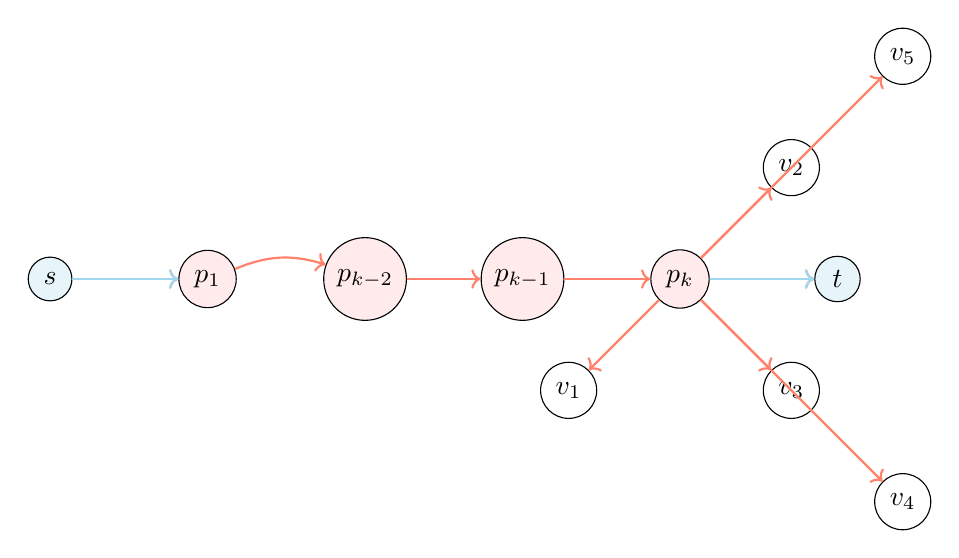
\begin{tikzpicture}[node distance=2cm, auto]
    % Define colors
    \definecolor{myblue}{RGB}{135,206,235}
    \definecolor{mypink}{RGB}{255,204,204}
    \definecolor{myred}{RGB}{255,99,71}
    
    % Nodes
    \node[draw,circle,fill=myblue!20] (s) {$s$};
    \node[draw,circle,fill=mypink!40] (p1) [right of=s] {$p_1$};
    \node[draw,circle,fill=mypink!40] (pk-2) [right of=p1] {$p_{k-2}$};
    \node[draw,circle,fill=mypink!40] (pk-1) [right of=pk-2] {$p_{k-1}$};
    \node[draw,circle,fill=mypink!40] (pk) [right of=pk-1] {$p_k$};
    \node[draw,circle,fill=myblue!20] (t) [right of=pk] {$t$};
    \node[draw,circle,fill=white] (v2) [above right of=pk] {$v_2$};
    \node[draw,circle,fill=white] (v1) [below left of=pk] {$v_1$};
    \node[draw,circle,fill=white] (v3) [below right of=pk] {$v_3$};
    \node[draw,circle,fill=white] (v4) [below right of=v3] {$v_4$};
    \node[draw,circle,fill=white] (v5) [above right of=v2] {$v_5$};
    
    % Edges
    \path[->,thick,draw=myred!80]
        (s) edge node {} (p1)
        (p1) edge[bend left=20] node {} (pk-2)
        (pk-2) edge node {} (pk-1)
        (pk-1) edge node {} (pk)
        (pk) edge node {} (t);
    \path[->,thick,draw=myblue!80]
        (s) edge node {} (p1)
        (pk) edge node {} (t);
    \path[->,thick,draw=myred!80]
        (pk) edge node {} (v2)
        (pk) edge node {} (v1)
        (pk) edge node {} (v3)
        (pk) edge node {} (v4)
        (pk) edge node {} (v5);
\end{tikzpicture}

\caption{Why $\langle s, p_1, \ldots, p_{k - 1} \rangle$ must be a most degree-central shortest path between $s$ and $p_{k - 1}$ if $\mathcal{N}(\langle s, p_1, \ldots, p_{k}, t\rangle)$ is a most degree-central shortest path between $s$ and $t$.}
\end{document}